\begin{figure}[t]
\centering
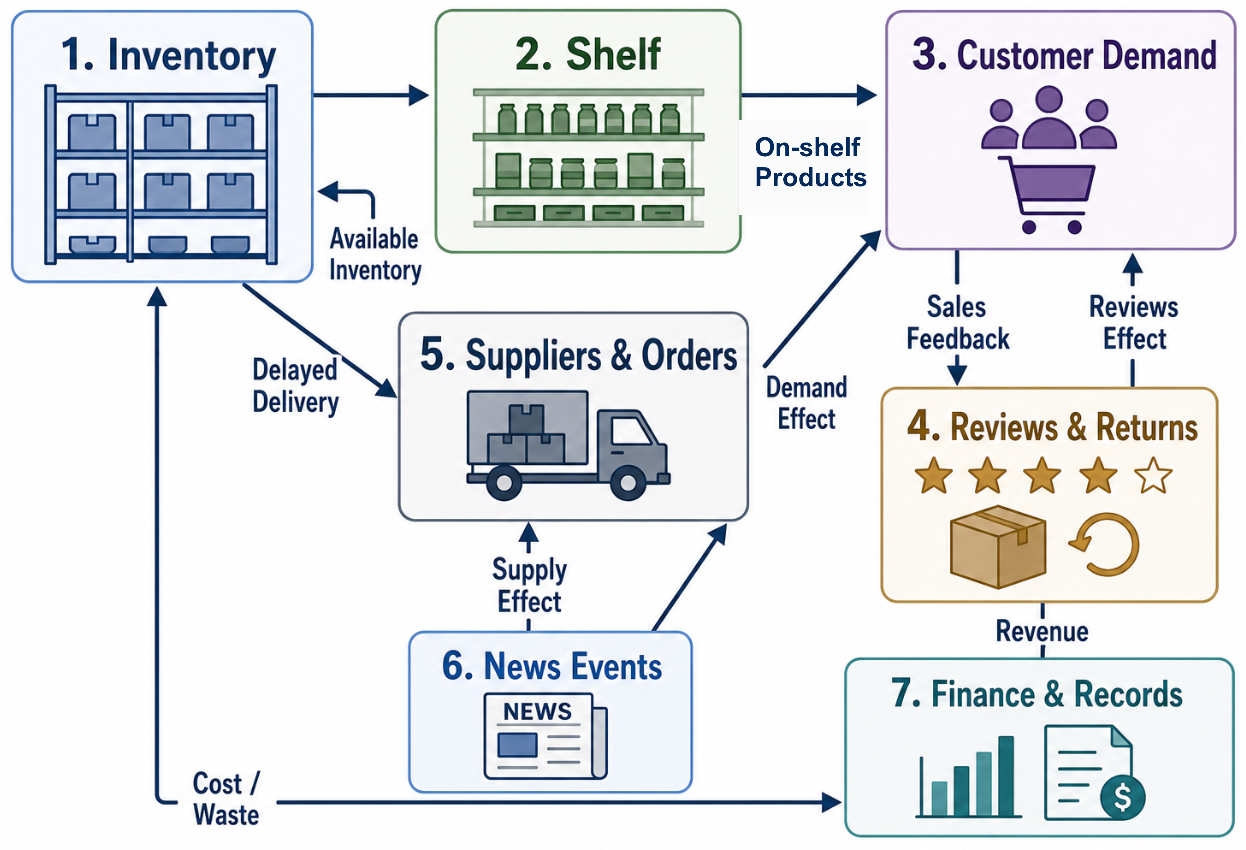
\includegraphics[width=\columnwidth]{figures/retailbench_first_page.pdf}
\caption{Overview of the RetailBench simulation environment. Inventory, shelf assortment, customer demand, suppliers and orders, reviews and returns, news events, and finance and records are coupled in this environment.}
\label{fig:retailbench_environment}
\vspace{-2mm}
\end{figure}

Large language models (LLMs), particularly when equipped with reasoning and tool-use capabilities, have achieved strong performance on short-horizon, structured tasks such as code editing, mathematical problem solving, complex information retrieval, and web interaction \citep{swe-bench, hle, omni-olpc, mialon2023gaiabenchmarkgeneralai, browsecomp, webarenarea, mind2web, tbench_2025}. As these benchmarks become increasingly saturated, the central question in agent evaluation is shifting from isolated task completion to sustained autonomy: can LLM agents pursue persistent objectives, adapt to evolving feedback, and recover from imperfect prior decisions over extended horizons?

Existing evidence suggests that this remains a major challenge. Recent studies show that even state-of-the-art agents often fail to maintain coherent strategies across long interactions, especially when local errors compound through delayed consequences and reshape future state distributions \citep{amodei2024machines, kwa2025measuringaiabilitycomplete, metr2025measuring, nof1, andonlabs2025vendingbench2, backlund2025vendingbenchbenchmarklongtermcoherence}. In response, benchmarks such as UltraHorizon, OdysseyBench, and HeroBench have begun to evaluate agents in temporally extended and more realistic environments \citep{utltabench,odysseybenchevaluatingllmagents,herobenchbenchmarklonghorizonplanning}. These efforts point to a broader methodological need: agent benchmarks should move beyond isolated task completion and evaluate whether agents can maintain persistent objective alignment and stable behavioral consistency in realistic long-horizon settings.

Retail business operation provides a natural testbed for this form of long-horizon agency. A store operator must repeatedly monitor inventory and cash flow, interpret historical sales and customer feedback, forecast future demand, and decide pricing, replenishment, and assortment actions whose effects may emerge only after several days. Prior work has studied related components, including retail and promotion simulation \citep{xia2023retailsynth,xia2024simulationretailpromotions}, transaction and demand modeling \citep{wang2025freshretailnet,tkachuk2024consumertransactions}, online shopping \citep{wang2025shoppingbench,3webshopscalablerealworldweb}, and inventory or order-fulfillment control \citep{OFCOURSE,inventory,leluc2023marlimmultiagentreinforcementlearning,invagentlargelanguagemodel,aimbenchevaluatingdecisionmakingbiases}. Yet these benchmarks typically isolate individual subproblems and do not capture the coupled, closed-loop dynamics of real business operation. As a result, the community lacks an open, real-data-grounded benchmark for evaluating tool-using LLM agents under diverse operational pressures over extended horizons.

We introduce \textit{RetailBench}, a controlled simulator for single-store supermarket operation grounded in real retail product and sales signals. In \textit{RetailBench}, agents repeatedly make pricing, replenishment, supplier-selection, information-acquisition, memory-management, and day-termination decisions while facing delayed deliveries, inventory aging, stockouts, customer reviews, returns, and financial constraints.

Our contributions are threefold:
\begin{itemize}[leftmargin=*]
    \item \textbf{A long-horizon retail environment.} We introduce \textit{RetailBench}, a data-grounded benchmark that evaluates LLM agents under coupled pricing, inventory, supplier, feedback, and financial dynamics.
    \item \textbf{An evaluation of current agent systems.} We benchmark representative agent frameworks and state-of-the-art LLMs, showing that current agents remain far from stable, high-performing long-horizon operational policies.
    \item \textbf{A systematic failure analysis.} We identify three recurring failure modes: \textbf{incomplete evidence acquisition}, \textbf{surface-level decision making}, and \textbf{lack of a consistent long-horizon policy}.
\end{itemize}